\chapter{SMING}\label{sec:sming}
Um weitere Sensoren einfach ohne Verdrahtung ins Messsystem aufzunehmen, setzen wir auf das Sming. Das Sming wurde durch Daniel Meer in seiner Master Thesis entwickelt. Er beschreibt in der Thesis das Sming wie folgt: \textit{Der TXW51 ist ein kleiner und energiesparender Sensorknoten, der als Basis für zukünftige Projekte verwendet werden kann. Er kommuniziert über Bluetooth Smart und enthält einen Sensor zur Messung der Beschleunigung. Die Firmware kann einfach für neue Anforderungen modifiziert werden.}\cite{meer:masterthesis}

\begin{figure}[hbtp]
	\center
	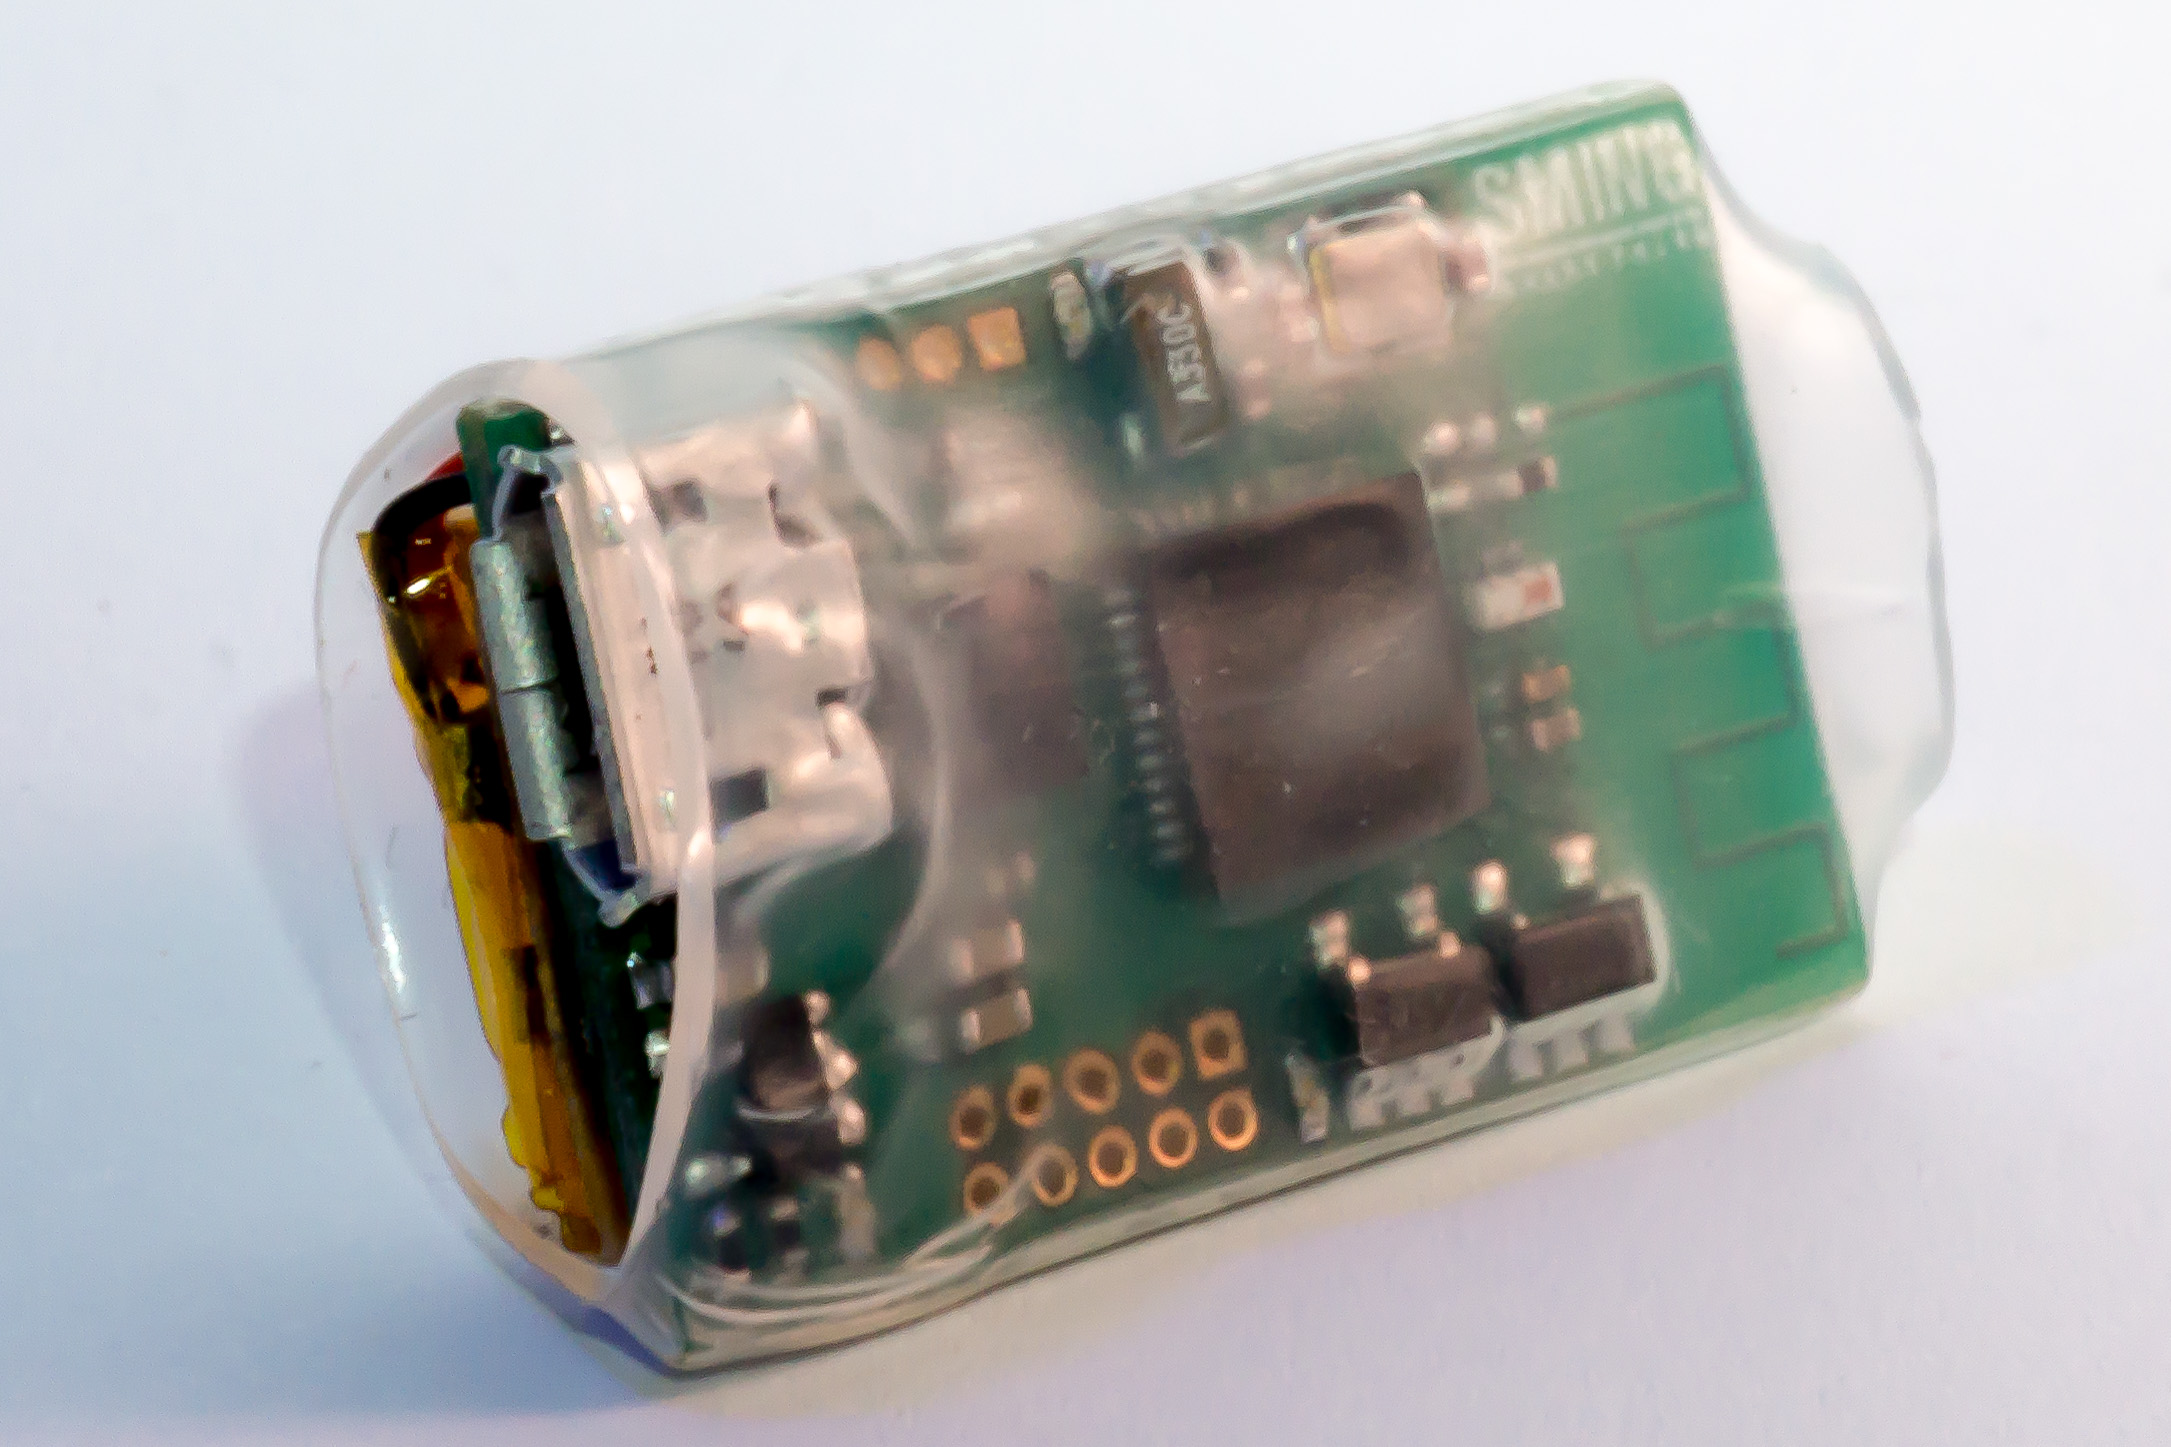
\includegraphics[width=10cm]{bilder/foto-6.jpg}
	\caption{Foto Sming mit Akku bestückt}
	\label{fig:sming}
\end{figure}

Für unser Projekt ist vorallem die Erweiterbarkeit des Sming sehr interessant. Dies weil beliebige Senosoren über I2C angesprochen werden können.

Um die angepasste Firmware zu testen, nutzen wir das von Bluegiga erhältlich BLE-Gui. Dies ermöglichte uns die Arbeit aufzuteilen, so dass auch ohne programmieren des Gateways die Änderungen an der Firmware getestet werden konnten. Um die bestehende Software zu testen, war dies zum Teil aber nicht optimal, weil, um einen höheren Datendurchsatz zu erreichen, wurden die Messwerte des Beschleunigungssensor in einer Charakteristik zusammengefasst.

%Hier nochmals die wichtigsten Eigenschaften:

%\begin{itemize}
%	\itemsep 1pt \parskip 0pt \parsep 0pt
%	\item Kommunikation über Bluetooth 4.0
%	\item Werte werden über BLE GATT gelesen und geschrieben 
%	\item Speziell wissenswert: Messungen werden per PUSH über Bluetooth CCID Feature gesendet, Details siehe Beschreibung BLED112
%	\item Bluetooth Device Name ist bei allen Smings von der BFH Burgdorf:  TXW51
%	\item Grundsätzlich sind die Attribute des SMINGS in drei Gruppen unterteilbar:
%	\begin{itemize}
%		\itemsep 1pt \parskip 0pt \parsep 0pt
%		\item Beginnend mit \url{DEVICE_INFO}: diverse einfache Textfelder, die auch selber nach gutdünken beschrieben werden können.
%		\item Beginnend mit LSM330: Die entsprechenden Einstellung und Werte des LSM330-Sensors (Kombinierter Gyro-,Accelometer- und Temperatur-Sensor)
%		\item Beginnend mit MEASURE: Die entsprechenden Funktionen, um die asynchrone Messung via Bluetooth Push zu konfigurieren (Dauer), zu starten, zu stoppen und auch von Hand den letzten Messwert abzufragen.
		
%	\end{itemize}
%	\item Tipp: Über das Demo-Tool von Bluegiga kann händisch mit dem SMING verbunden und Attribute gelesen/geschrieben werden.
	
%	\item Messwert-Attribut: Zum Optimieren der Performance sind auf dem Messwert-Attribut oft bis zu drei Messwerte binär aneinandergereit vorhanden. Das Decodieren des Wertes wird im Demo-Script von Zeile 319 bis 345 gemacht.
	
%	\item Java-Beispielcode für Kommunikation ist ebenfalls vorhanden,siehe gezippter Source der Demo-Android App von Daniel Meer auf Google Drive. Dort wird aber mit den Android Bluetooth Stack gearbeitet und nicht mit dem Bluegiga, weswegen sich das leider nicht ganz eins zu eins kopieren lässt. 
	
%	\item Hinweis: das CCID wird von Android im Gegensatz zu Bluegiga als Funktion abstrahiert.
%\end{itemize}


\clearpage
\section{BLE-I2C Bridge}
\label{bleI2cBridge}

Das Sming verfügt über den Erweiterungsheader die Möglichkeit I2C Sensoren anzusprechen. Um diese Funktion zu nutzen, muss die Firmware des Smings erweitert werden. Dies ist nicht Straight-Forward, weil für die Entwicklung in C und das Deployment auf den NRF51 spezielle Hardware und Software erforderlich ist. Um dieses Problem zu umgehen, wurde die BLE-I2C Bridge entwickelt. Sie soll dazu dienen, dass vom IoT-Gateway via Sming I2C Sensoren und Aktoren angesprochen werden können. Somit muss für einen neuen Sensor die Firmware der Smings nicht mehr angerührt werden. Dafür muss aber das IoT-Gateway programmiert werden. Dieses lässt sich je nach Gateway Typ leicht über Ethernet oder USB programmieren. Auch die Softwareentwicklung in JavaScript sollte den meisten Entwickler in der Informatik-Branche weniger schwer fallen als dies bei C der Fall ist.

\begin{figure}[hbtp]
    \center
    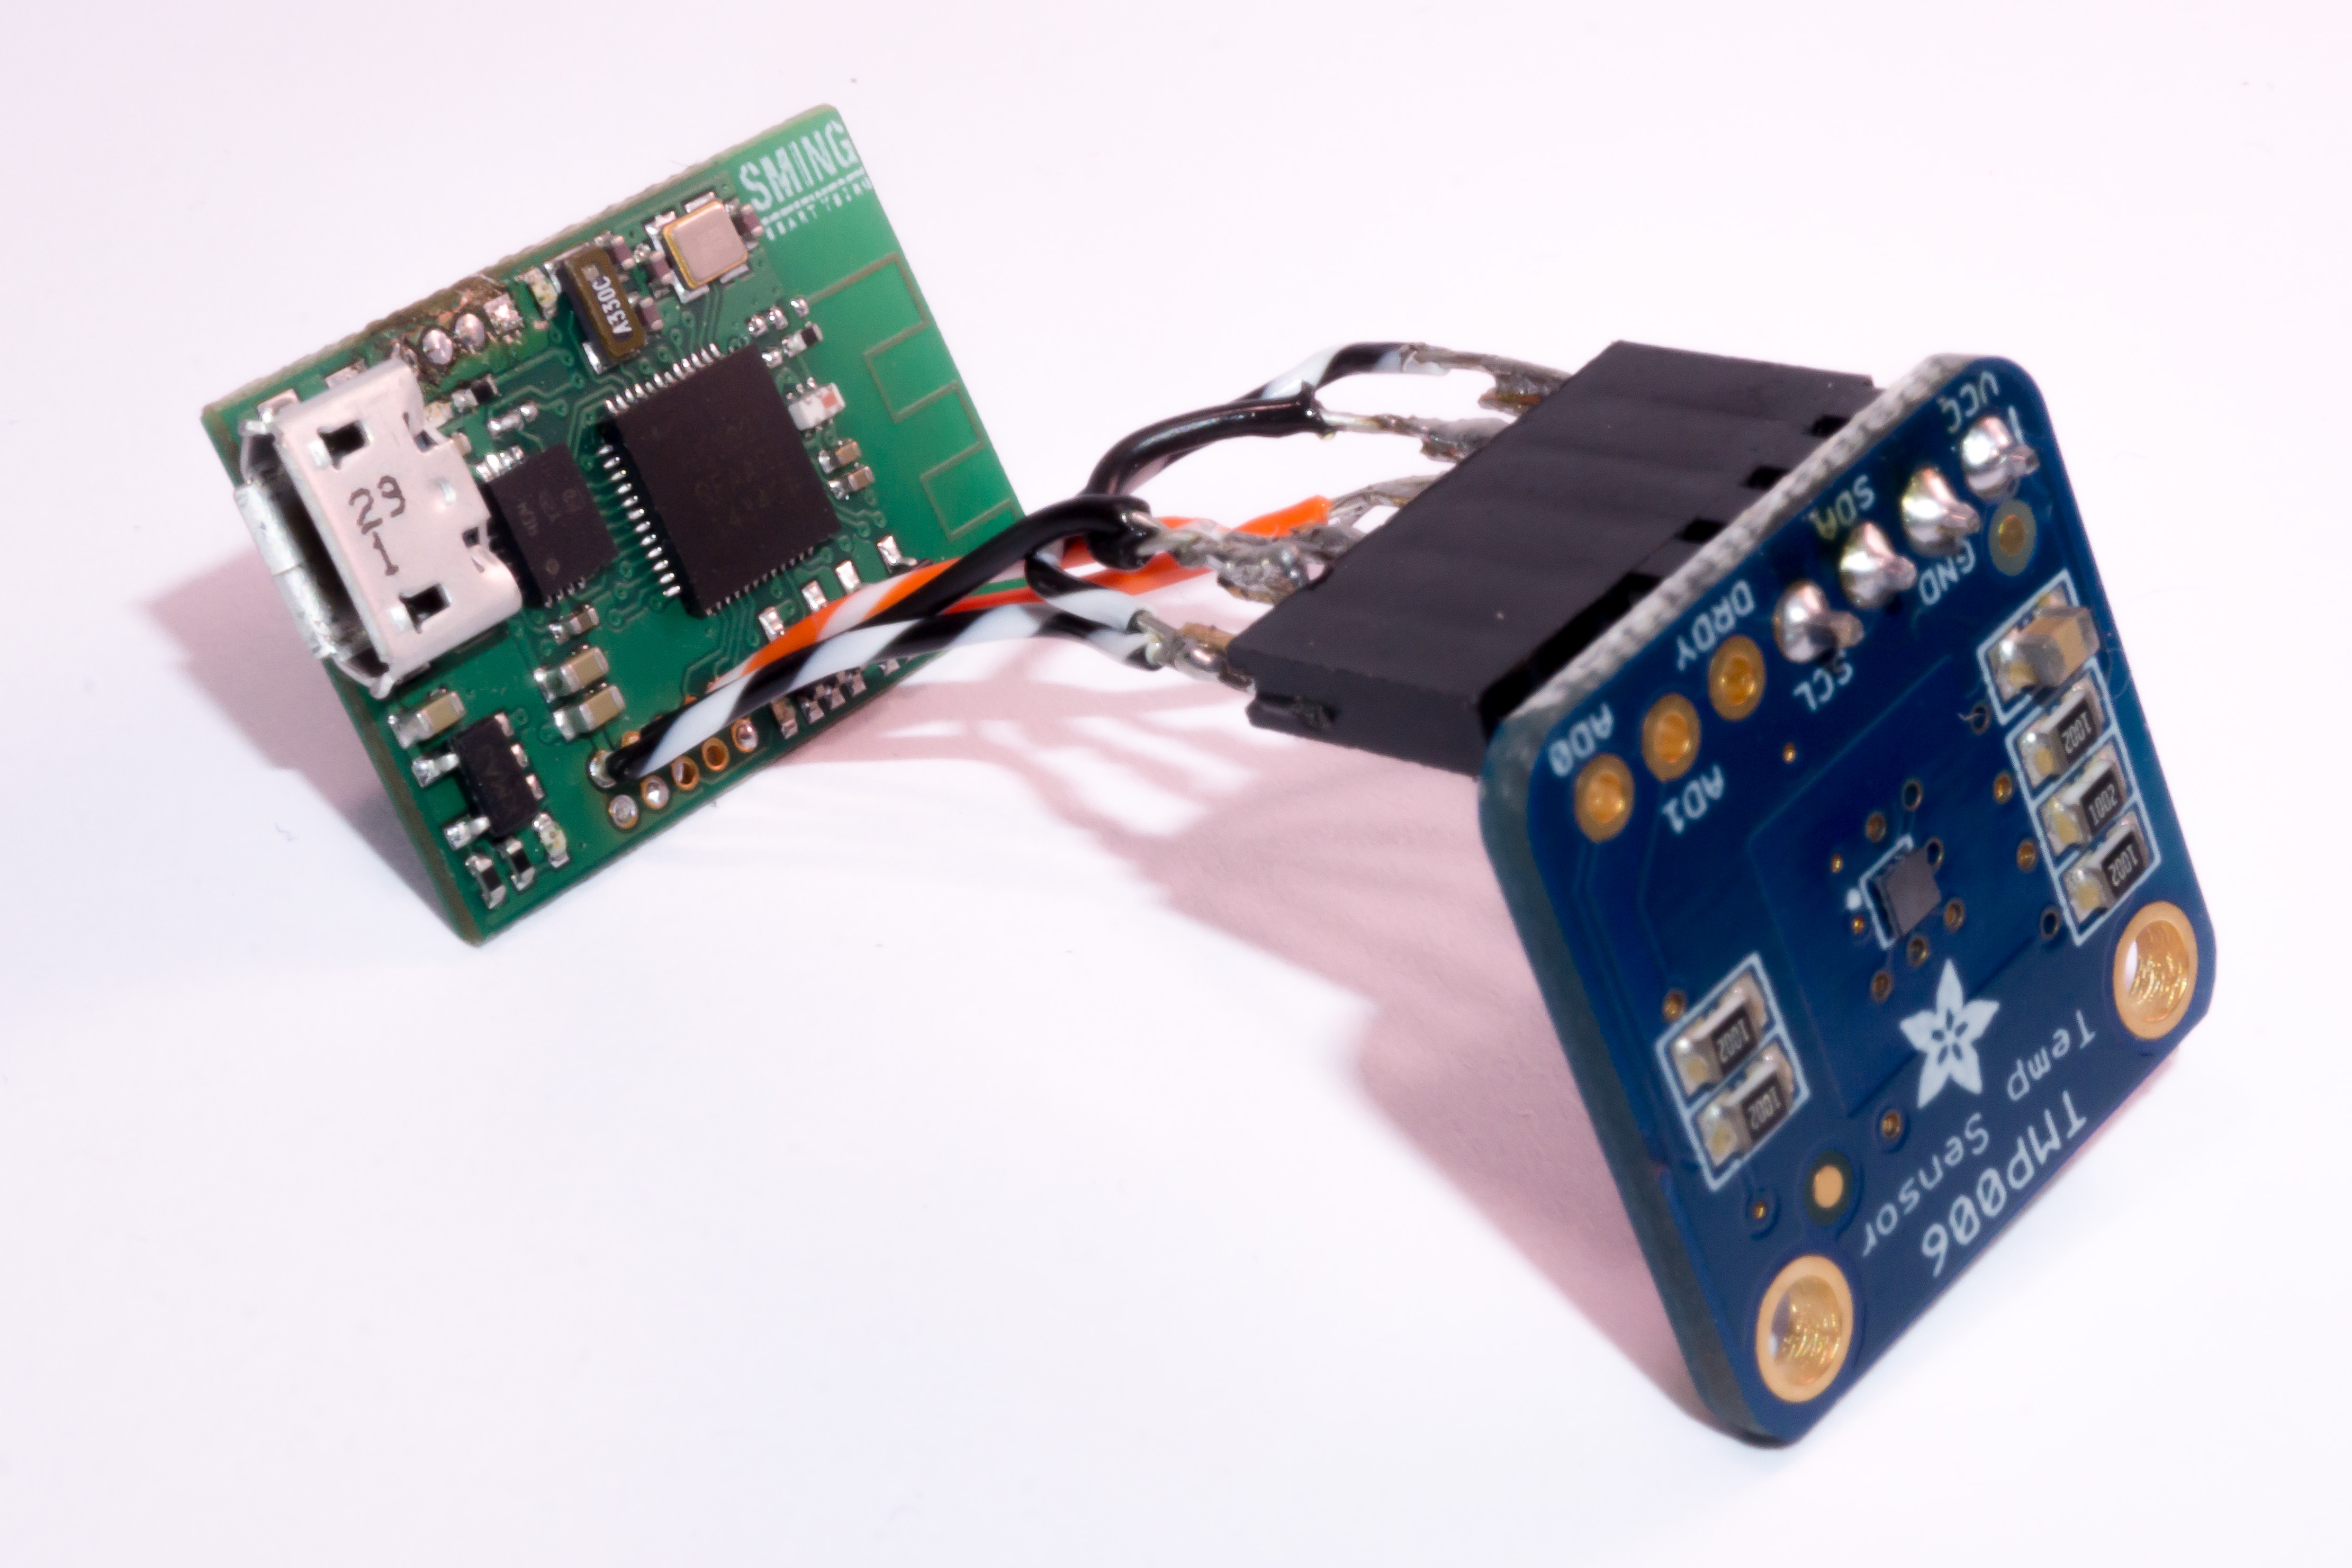
\includegraphics[width=\textwidth]{bilder/foto-2.jpg}
    \caption{Sming mit über I2C Bridge abfragbaren TMP06 Sensor}
    \label{fig:sming_mit_tmp06}
\end{figure}

\clearpage
\section{Implementation}
\label{bleI2cImplementation}

Für die BLE-I2C Bridge wurde ein eigener BLE-Service aufgesetzt. Dieser wird in den nachfolgenden Tabellen beschrieben:

%\begin{table}[h]
%\centering
\begin{tabularx}{\textwidth}{|l|X|}
\hline
Name & I2C Service                                       \\
\hline
Beschreibung & Ein Service für I2C Devices über BLE anzusprechen \\
\hline
UUID	&    0x8EDF0500-67E5-DB83-F85B-A1E2AB1C9E7A  \\
\hline                                            
\end{tabularx}
%\caption{Ble I2C Service}
%\label{tab:bleI2cService}
%\end{table}

Folgende Charakteristiken stehen bei dem Service zur Verfügung:

%\begin{table}[h]
%\centering
\begin{tabularx}{\textwidth}{|l|X|}
\hline
Name & I2C Device Adress                                   \\
\hline
Beschreibung & Wird verwendet um die I2C Adresse des Sensor (oder Aktor) im Sming einzustellen. \\
\hline
UUID	&    0x8EDF0501-67E5-DB83-F85B-A1E2AB1C9E7A  \\
\hline     
Anzahl Byte	&    1  \\
\hline      
Zugriffsrechte	&   R/W  \\
\hline        
Wertebereich	&   0x00 .. 0x7F \\
\hline          
Wertebereich	&   0x00 \\
\hline                                     
\end{tabularx}
%\caption{Ble I2C Device Adress Charakteristik}
%\label{tab:bleI2cDeviceAdress}
%\end{table}

%\begin{table}[h]
%\centering
\begin{tabularx}{\textwidth}{|l|X|}
\hline
Name & I2C Device Register                                  \\
\hline
Beschreibung & Wird verwendet um das I2C Register des Sensor (oder Aktor) im Sming einzustellen, auf welches geschrieben oder von welchem gelesen werden soll. \\
\hline
UUID	&    0x8EDF0502-67E5-DB83-F85B-A1E2AB1C9E7A  \\
\hline     
Anzahl Byte	&    1  \\
\hline      
Zugriffsrechte	&   R/W  \\
\hline        
Wertebereich	&   0x00 .. 0xFF \\
\hline          
Wertebereich	&   0x00 \\
\hline                                     
\end{tabularx}
%\caption{Ble I2C Device Register Charakteristik}
%\label{tab:bleI2cDeviceRegister}
%\end{table}

%\begin{table}[h]
%\centering
\begin{tabularx}{\textwidth}{|l|X|}
\hline
Name & I2C Read Length                              \\
\hline
Beschreibung & Wird verwendet um die Anzahl Bytes einzustellen, welche von dem eingestellten Register gelesen werden. \\
\hline
UUID	&    0x8EDF0503-67E5-DB83-F85B-A1E2AB1C9E7A \\
\hline     
Anzahl Byte	&    1  \\
\hline      
Zugriffsrechte	&   R/W  \\
\hline        
Wertebereich	&   0x00 .. 0xFF \\
\hline          
Wertebereich	&   0x00 \\
\hline                                     
\end{tabularx}
%\caption{Ble I2C Device Read Length Charakteristik}
%\label{tab:bleI2cDeviceReadLength}
%\end{table}

%\begin{table}[h]
%\centering
\begin{tabularx}{\textwidth}{|l|X|}
\hline
Name & I2C Read Length                              \\
\hline
Beschreibung & Wird verwendet um die eingestellte Anzahl Bytes von dem eingestellten Register zu lesen oder die in der Charakteristik mitgegebene Anzahl Bytes auf das angegebene Register zu schreiben.\\
\hline
UUID	&    0x8EDF0504-67E5-DB83-F85B-A1E2AB1C9E7A \\
\hline     
Anzahl Byte	&    1 .. 10  \\
\hline      
Zugriffsrechte	&   R/W  \\
\hline        
Wertebereich	&   0x00 .. 0xFF \\
\hline          
Wertebereich	&   0x00 \\
\hline                                     
\end{tabularx}
%\caption{Ble I2C Value Charakteristik}
%\label{tab:bleI2cValue}
%\end{table}